\section{Proposed System}
\label{method}

\begin{figure*}[t]
  \centering
  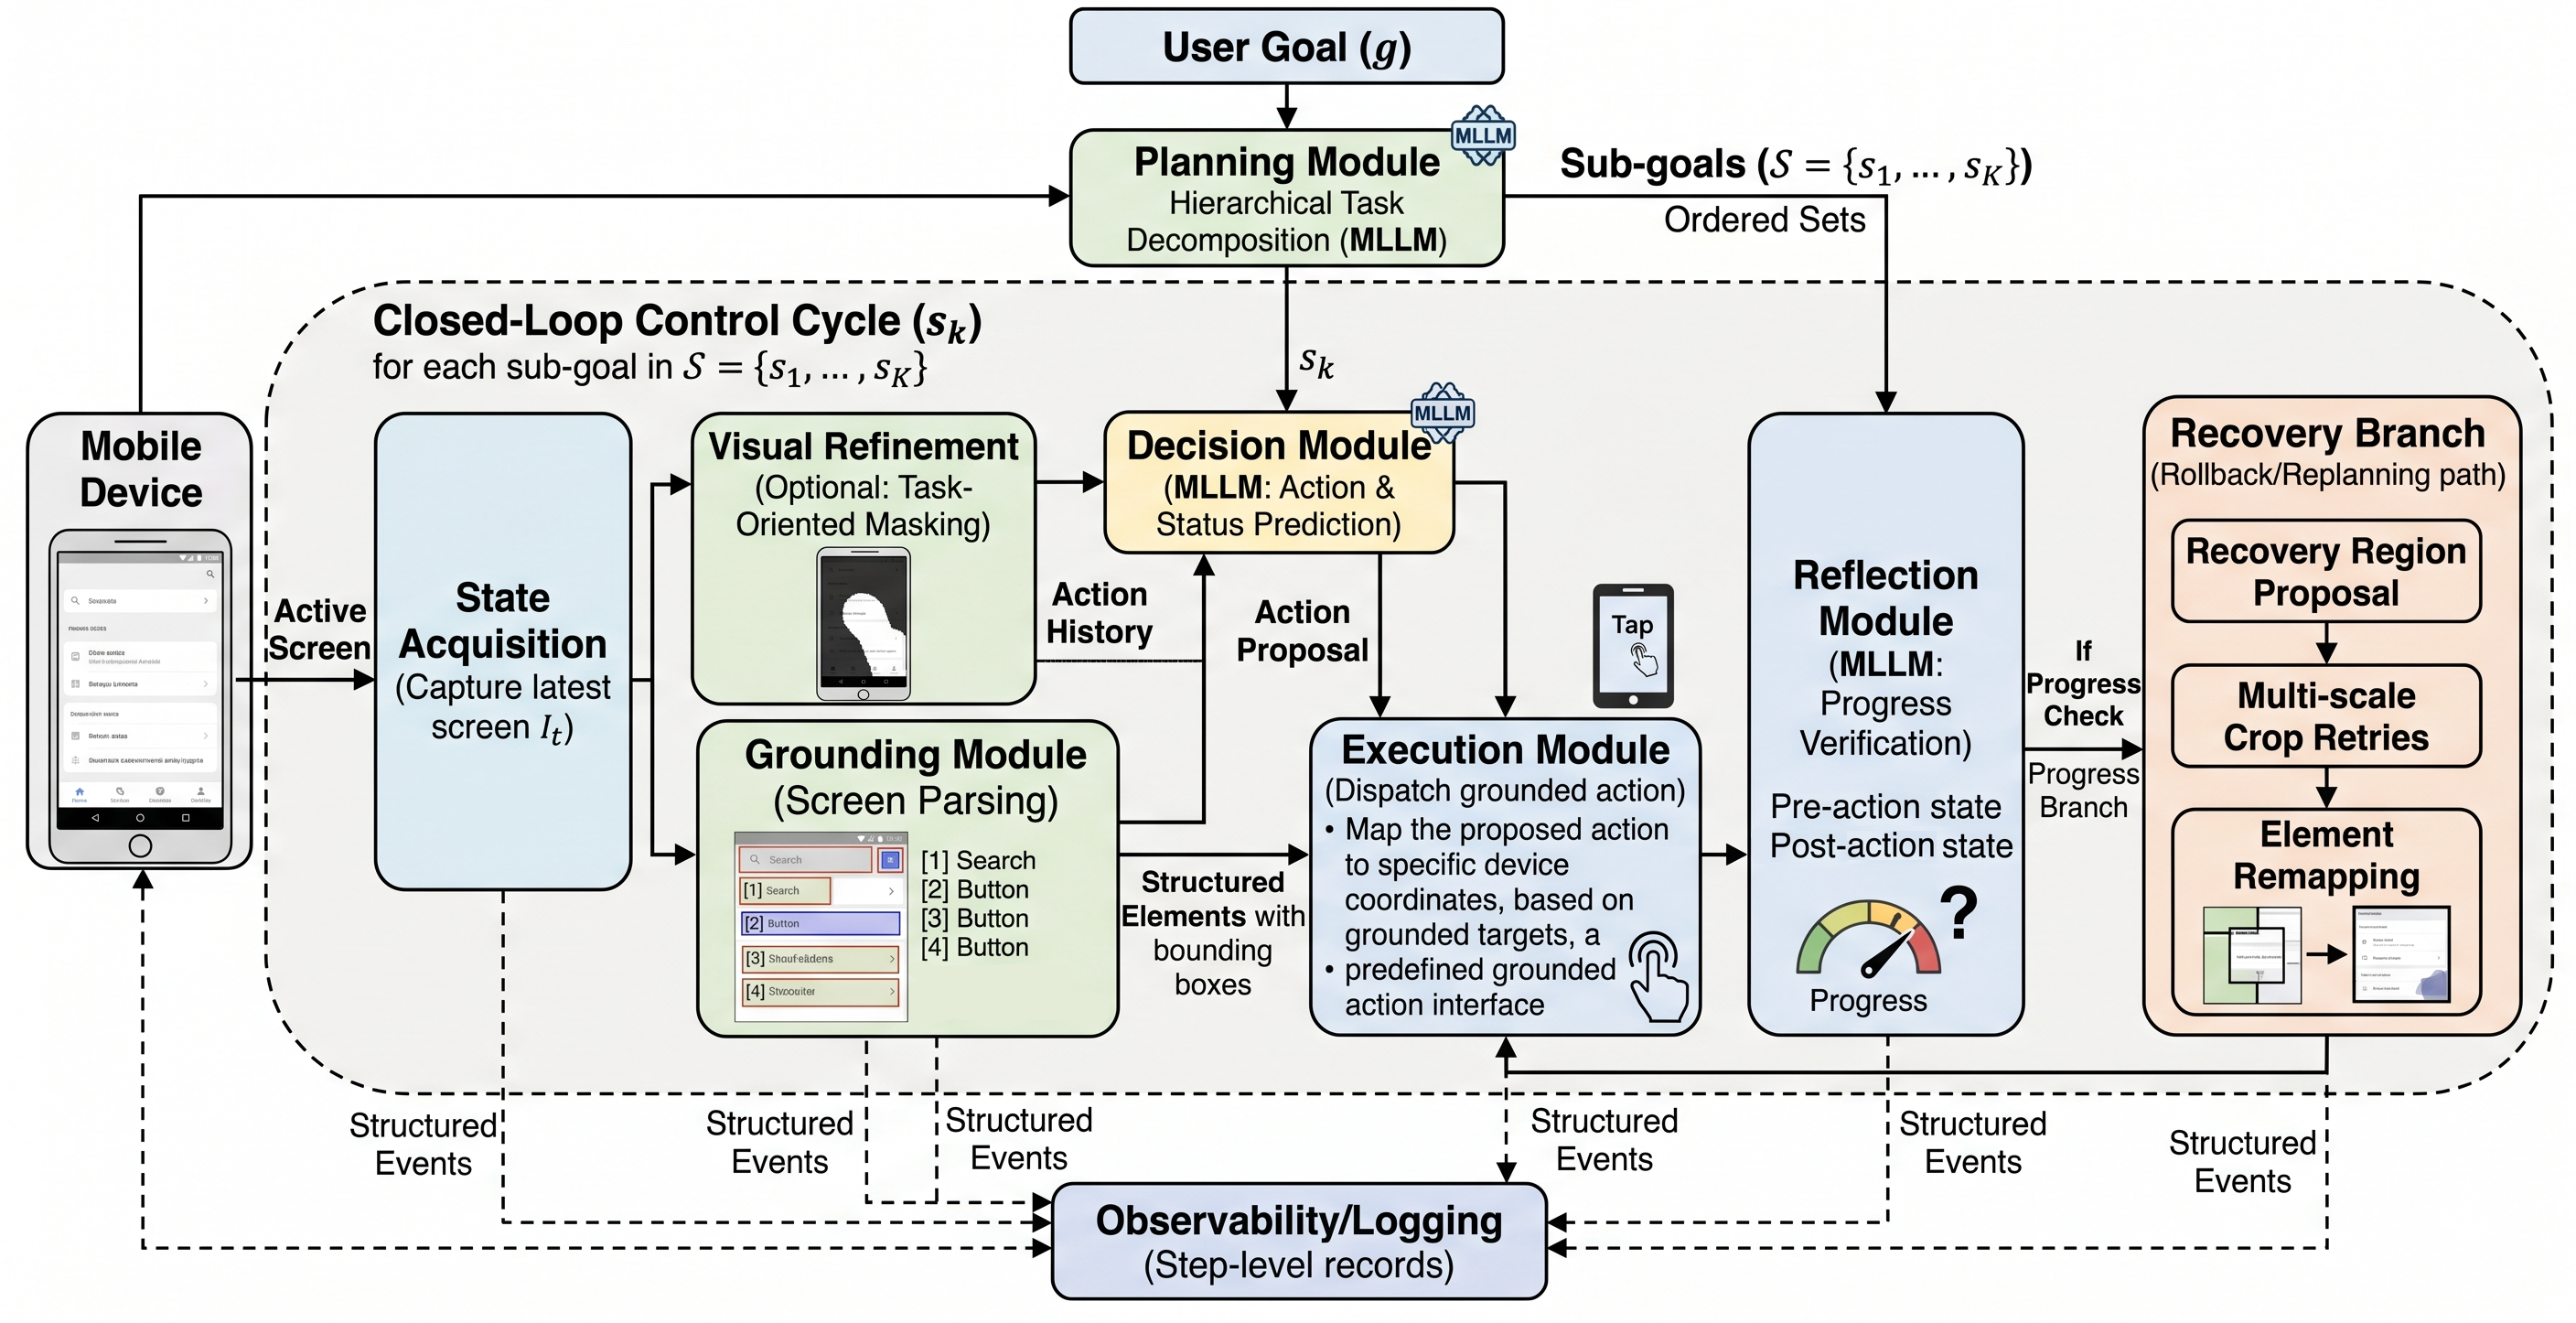
\includegraphics[width=\textwidth]{image/system-overview-crop_2.png}
  \caption{End-to-end architecture of the screenshot-only mobile GUI agent. Given a user goal, the system plans sub-goals and iteratively performs grounded action execution on the current screen. Each step optionally applies visual refinement, grounds decisions to detected UI elements, executes on-device actions, and reflects on progress. Recovery paths (rollback, region proposal, and multi-scale retry) are triggered when interactions stall or fail.}
  \label{fig:system_overview}
\end{figure*}

\subsection{Overview}
We design a screenshot-only mobile GUI agent that closes the perception--action loop with explicit grounding. Given a user goal, the system performs hierarchical task decomposition into sub-goals, enumerates a unified action space, and constructs a GUI state from two sources: (i) a visual parser that returns UI elements with bounding boxes, and (ii) linguistic context summarizing past actions and the active sub-goal. The decision module selects an element index rather than free-form coordinates; this index is mapped to device coordinates for execution. After each action, a reflection step verifies progress using an MLLM-based check and decides whether to proceed, replan, or terminate.

The design emphasizes interface reliability and observability. Each step emits structured events, enabling debugging and analysis of failure modes such as missed detections, incorrect grounding, or stalled progress. This overview sets up the system architecture and implementation details presented next.

\subsection{System Architecture}
\paragraph{Design Principle}
The architecture is designed around a stable separation of concerns: high-level reasoning is delegated to the MLLM, while action validity is enforced by explicit grounding and deterministic execution interfaces. This separation is unlikely to change across model versions because it addresses a structural reliability issue in GUI automation: language models are strong at planning but error-prone when unconstrained at the pixel-action boundary.

\paragraph{Pipeline Structure}
Given a user goal $g$ and an initial screenshot $I_0$, the system first produces an ordered set of sub-goals $\mathcal{S}=\{s_1,\dots,s_K\}$. For each active sub-goal $s_k$, the agent runs a closed-loop control cycle over the current screenshot $I_t$:
\begin{enumerate}
    \item \textbf{State acquisition:} capture the latest mobile screen as an RGB screenshot.
    \item \textbf{Optional visual refinement:} apply task-oriented masking to reduce irrelevant visual regions.
    \item \textbf{Action decision:} predict a next action proposal and sub-goal status from the current state and action history.
    \item \textbf{Grounding:} parse the screen into structured UI elements (with normalized bounding boxes and metadata).
    \item \textbf{Execution:} dispatch the grounded action to the device.
    \item \textbf{Reflection:} verify whether the action produced observable progress; otherwise trigger recovery.
\end{enumerate}


\begin{table*}[t]
  \centering
  \small
  \caption{Module interfaces and recovery mechanisms. Each row summarizes one pipeline component; interface and failure details are grouped to improve readability.}
  \label{tab:module_interfaces}
  \renewcommand{\arraystretch}{1.15}
  \setlength{\tabcolsep}{4pt}
  \begin{tabularx}{\textwidth}{@{}l
      >{\raggedright\arraybackslash}X
      >{\raggedright\arraybackslash}X@{}}
    \toprule
    \textbf{Module} & \textbf{Interface} & \textbf{Failure and recovery} \\
    \midrule
    Planner &
    \textbf{Input:} user goal $g$, initial screenshot $I_0$. \newline
    \textbf{Output:} ordered sub-goals $\mathcal{S}=\{s_1,\dots,s_K\}$. &
    \textbf{Signal:} infeasible goal or decomposition failure. \newline
    \textbf{Recovery:} abort task or request user clarification. \\
    \addlinespace
    Achiever &
    \textbf{Input:} active sub-goal $s_k$, screenshot $I_t$, action history. \newline
    \textbf{Output:} next action, sub-goal status, optional rollback index. &
    \textbf{Signal:} invalid sequence or rollback request. \newline
    \textbf{Recovery:} propose recovery region; enter reflection branch. \\
    \addlinespace
    Grounder &
    \textbf{Input:} screenshot $I_t$ (optionally masked). \newline
    \textbf{Output:} UI elements with normalized boxes and metadata. &
    \textbf{Signal:} missed or mis-grounded elements. \newline
    \textbf{Recovery:} multi-scale crop retries and localized re-attention. \\
    \addlinespace
    Executor &
    \textbf{Input:} grounded action (element index $\rightarrow$ coordinates). \newline
    \textbf{Output:} on-device interaction (tap, type, scroll). &
    \textbf{Signal:} off-screen, occluded, or unclickable target. \newline
    \textbf{Recovery:} scroll to reveal, remap crop coordinates, or report error. \\
    \addlinespace
    Reflection &
    \textbf{Input:} pre/post-action states and attempted action. \newline
    \textbf{Output:} progress verdict (proceed, replan, terminate). &
    \textbf{Signal:} no visual change or stalled loop. \newline
    \textbf{Recovery:} rollback history and force sub-goal replanning. \\
    \bottomrule
  \end{tabularx}
\end{table*}


The loop terminates when the current sub-goal is completed or a step budget is exhausted; execution then advances to the next sub-goal until all sub-goals are processed.

\paragraph{Grounded Action Interface}
The key architectural choice is to represent interaction targets as detected UI elements instead of free-form coordinate generation. Concretely, the decision module operates over a structured action space (e.g., click/type/scroll with element-conditioned targets), and the executor converts grounded targets into device-level interactions. This interface improves controllability, enables post-hoc inspection of action rationale, and reduces coordinate hallucination risk in cluttered screens.

\paragraph{Recovery and Replanning Path}
To handle execution failures and non-progress states, the architecture includes a recovery branch. When reflection or decision signals indicate rollback, the agent proposes a broad recovery region, optionally performs multi-scale crop-based retries, and remaps successful crop-localized elements back to original-screen coordinates before dispatch. This design preserves correctness at the device interface while allowing local re-attention around uncertain regions.

\paragraph{Event-Driven Observability}
Each step is represented as structured state transitions (planning, sub-goal execution, reflection, replanning, completion/failure) with step-level records. This event-oriented design supports reproducibility, failure analysis, and ablation studies without changing the core control loop, making it a durable systems contribution beyond any single model backend.

\paragraph{Modular Extensibility}
The architecture intentionally keeps model-dependent components replaceable:
\begin{itemize}
    \item The planner/achiever can be swapped across MLLM providers.
    \item The screen parser can be replaced or upgraded without changing downstream executor contracts.
    \item Reflection policies can evolve (e.g., stronger verification or uncertainty-aware checks) while preserving the same loop structure.
\end{itemize}
These invariants make the system robust to rapid changes in foundation models and parsing tools.

Figure~\ref{fig:system_overview} summarizes the end-to-end control flow, including planning, the per-step execution loop, and recovery/replanning edges. Table~\ref{tab:module_interfaces} defines module-level interfaces and recovery behavior.


\subsection{Implementation Details}
We keep implementation details concise and emphasize reproducibility. The system is implemented as a modular backend with a streaming API and a lightweight frontend for observability. Planning, action selection, and verification are performed via MLLM calls using a Gemini API key, while grounded actions are dispatched through ADB to the device. Each step emits structured events and logs that enable replay and failure analysis. \textcolor{red}{TODO: include exact model name, prompt templates, and decoding settings used in experiments.}

Table~\ref{tab:impl_summary} summarizes key components and minimal implementation details relevant for reproducibility.

\begin{table}[t]
  \centering
  \small
  \caption{Implementation summary (compact).}
  \label{tab:impl_summary}
  \renewcommand{\arraystretch}{1.1}
  \setlength{\tabcolsep}{6pt}
  \begin{tabularx}{\linewidth}{@{}lX@{}}
    \toprule
    \textbf{Component} & \textbf{Notes} \\
    \midrule
    Perception & Screenshot parsing to UI elements with normalized boxes. \\ \textcolor{red}{TODO: parser version, thresholds.} \\
    Grounding & Element index mapped to pixel coordinates via device resolution. \\ \textcolor{red}{TODO: preprocessing.} \\
    Decision/Reflection & MLLM planning and verification (Gemini). \\ \textcolor{red}{TODO: model + prompts.} \\
    Execution & ADB tap/type/scroll dispatch from grounded targets. \\ \textcolor{red}{TODO: command timing.} \\
    Observability & Step-level logs and event stream for replay. \\ \textcolor{red}{TODO: logging locations.} \\
    \bottomrule
  \end{tabularx}
\end{table}
